\documentclass[10pt]{article}
\usepackage[utf8]{inputenc}
\usepackage[T1]{fontenc}
\usepackage{amsmath}
\usepackage{amsfonts}
\usepackage{amssymb}
\usepackage[version=4]{mhchem}
\usepackage{stmaryrd}
\usepackage{graphicx}
\usepackage[export]{adjustbox}
\graphicspath{ {./images/} }

\begin{document}

    The rotation curve of our Galaxy is determined using line-of-sight velocity measurements of neutral hydrogen (HI) clouds along various Galactic longitudes, observed through the 21 cm HI line. Consider an HI cloud with Galactic longitude $l$, located at a distance $R$ from the Galactic Centre (GC) and a distance $D$ from the Sun. Consider Sun to be at a distance $R_{0}=8.5 \mathrm{kpc}$ from the GC. Assume that both the Sun and the HI cloud are in circular orbits around the GC in the Galactic plane, with angular velocities $\Omega_{0}$ and $\Omega$, and rotational velocities $V_{0}$ and $V$, respectively.

    The line-of-sight velocity ( $V_{\mathrm{r}}$ ) and transverse velocity ( $V_{\mathrm{t}}$ ) components of the cloud, as observed from the Sun, can be expressed as
    
    $$
    \begin{gathered}
    V_{\mathrm{r}}=\left(\Omega-\Omega_{0}\right) R_{0} \sin l \\
    V_{\mathrm{t}}=\left(\Omega-\Omega_{0}\right) R_{0} \cos l-\Omega D
    \end{gathered}
    $$
    
    Seen from the North Galactic Pole, the Galactic rotation is clockwise. Throughout this problem, we shall take line-ofsight velocity to be positive when receding and clouds will be treated as point objects.\\
    (T06.1) In the graph provided on the Summary Answersheet, sketch $V_{\mathrm{r}}$ as a function of $D$ from $D=0$ to $D=2 R_{0}$ for two lines of sight defined by (i) $l=45^{\circ}$ and (ii) $l=135^{\circ}$. Label each of your lines/curves with the value of $l$.\\
    (T06.2) The graph below shows the average radial (solid, red curve) and transverse (dashed, blue curve) velocity components of stars at a distance of 100 pc from the Sun, plotted as a function of Galactic longitude.\\
    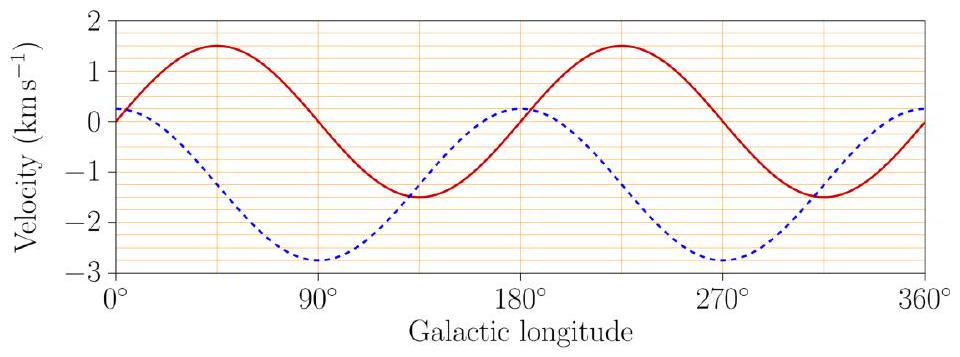
\includegraphics[max width=\textwidth, center]{2025_08_23_e94579452776a99c4850g-05}
    
    Using the graph, estimate the Sun's orbital period ( $P$ ) around the GC in mega-years (Myr).\\
    (T06.3) Jan Oort noted that in the solar neighbourhood ( $D \ll R_{0}$ ), the difference in angular velocities ( $\Omega-\Omega_{0}$ ) will be small, and hence, derived the following first order approximation for the line-ofsight and the transverse velocity components:
    
    $$
    \begin{aligned}
    & V_{\mathrm{r}}=A D \sin 2 l \\
    & V_{\mathrm{t}}=A D \cos 2 l+B D
    \end{aligned}
    $$
    
    where $A$ and $B$ are known as Oort's constants.\\
    Let us consider two cases:\\
    (I) the actual observed rotation curve of the Galaxy, and\\
    (II) the rotation curve is for a hypothetical scenario where the Galaxy is devoid of dark matter and the whole mass of the Galaxy is assumed to be concentrated at its centre.\\
    (T06.3a) Derive expressions for the radial gradient of the rotational velocity at the location of the Sun, $\left.\frac{d V}{d R}\right|_{R=R_{0}}$, for the two cases.\\
    (T06.3b) Express $A$ and $B$ in terms of $V_{0}, R_{0}$, and the radial gradient of rotational velocity at the location of the Sun, $\left.\frac{d V}{d R}\right|_{R=R_{0}}$.\\
    (T06.3c) The ratio $(A / B)$ of Oort's constants for the two given cases, (I) and (II), are defined as $F_{\mathrm{I}}$ and $F_{\mathrm{II}}$, respectively. Determine $F_{\mathrm{I}}$ and $F_{\mathrm{II}}$.


\end{document}